\documentclass[%
crop,%
tikz,%
convert={outext=.svg,command=\unexpanded{pdf2svg \infile\space../_static/\outfile}},%
multi=false%
]{standalone}%
\usepackage[utf8]{luainputenc}%
\usepackage[no-math]{fontspec}%
\defaultfontfeatures{%
    Numbers={OldStyle,Proportional},%
    Ligatures=TeX,%
    Extension=.ttf,%
}%
\setmainfont[%
UprightFont=*-Regular,%
ItalicFont=*-Italic,%
BoldFont=*-Bold,%
BoldItalicFont=*-BoldItalic,%
]{Raleway}%
\setsansfont[%
UprightFont=*-Regular,%
ItalicFont=*-Italic,%
BoldFont=*-Bold,%
BoldItalicFont=*-BoldItalic,%
]{Raleway}%
\usepackage[frenchmath]{mathastext}%
\usepackage{amsmath}%
\usepackage{amssymb}%
\usepackage{mathrsfs}%
\usepackage{mathtools}%
\usepackage{siunitx}%
\usepackage[siunitx]{circuitikz}%
\usetikzlibrary{calc,backgrounds,arrows.meta,patterns}%

\DeclareMathOperator{\sign}{sign}%

% Ensembles
\let\C\relax
\newcommand{\R}{\ensuremath{\mathbb{R}}} % Réel
\newcommand{\N}{\ensuremath{\mathbb{N}}} % Entiers naturels
% \newcommand{\C}{\ensuremath{\mathbb{C}}} % Complexes
\newcommand{\B}{\ensuremath{\mathscr{B}}} % Bus électriques
\newcommand{\Ch}{\ensuremath{\mathscr{C}}} % Charges
\renewcommand{\L}{\ensuremath{\mathscr{L}}} % Lignes
\renewcommand{\P}{\ensuremath{\mathscr{P}}} % Phases

% Phases
\newcommand{\arm}{\ensuremath{\mathrm{a}}}%
\newcommand{\brm}{\ensuremath{\mathrm{b}}}%
\newcommand{\crm}{\ensuremath{\mathrm{c}}}%
\newcommand{\nrm}{\ensuremath{\mathrm{n}}}%
\newcommand{\trm}{\ensuremath{\mathrm{t}}}%
\newcommand{\grm}{\ensuremath{\mathrm{g}}}%
\newcommand{\abrm}{\ensuremath{\mathrm{ab}}}%
\newcommand{\bcrm}{\ensuremath{\mathrm{bc}}}%
\newcommand{\carm}{\ensuremath{\mathrm{ca}}}%
\newcommand{\anrm}{\ensuremath{\mathrm{an}}}%
\newcommand{\bnrm}{\ensuremath{\mathrm{bn}}}%
\newcommand{\cnrm}{\ensuremath{\mathrm{cn}}}%
\newcommand{\atrm}{\ensuremath{\mathrm{at}}}%
\newcommand{\btrm}{\ensuremath{\mathrm{bt}}}%
\newcommand{\ctrm}{\ensuremath{\mathrm{ct}}}%
\newcommand{\ntrm}{\ensuremath{\mathrm{nt}}}%
\newcommand{\agrm}{\ensuremath{\mathrm{ag}}}%
\newcommand{\bgrm}{\ensuremath{\mathrm{bg}}}%
\newcommand{\cgrm}{\ensuremath{\mathrm{cg}}}%
\newcommand{\ngrm}{\ensuremath{\mathrm{ng}}}%
\newcommand{\abcrm}{\ensuremath{\mathrm{abc}}}%
\newcommand{\abcnrm}{\ensuremath{\mathrm{abcn}}}%

% Indices ou exposants
\newcommand{\cons}{\ensuremath{\mathrm{cons.}}}%
\renewcommand{\prod}{\ensuremath{\mathrm{prod.}}}%
\newcommand{\theo}{\ensuremath{\mathrm{th.}}}%
\newcommand{\const}{\ensuremath{\mathrm{const.}}}%

% Variables
\newcommand{\umax}{\ensuremath{U^{\max}}}%
\newcommand{\umaxnorm}{\ensuremath{U^{\max\,\text{norm.}}}}%
\newcommand{\umin}{\ensuremath{U^{\min}}}%
\newcommand{\uminnorm}{\ensuremath{U^{\min\,\text{norm.}}}}%
\newcommand{\unom}{\ensuremath{U^{\text{nom.}}}}%
\newcommand{\unomnorm}{\ensuremath{U^{\text{nom.}\,\text{norm.}}}}%
\newcommand{\uup}{\ensuremath{U^{\text{up}}}}%
\newcommand{\uupnorm}{\ensuremath{U^{\text{up}\,\text{norm.}}}}%
\newcommand{\uupprime}{\ensuremath{U^{\text{up}\,\prime}}}%
\newcommand{\udown}{\ensuremath{U^{\text{down}}}}%
\newcommand{\udownnorm}{\ensuremath{U^{\text{down}\,\text{norm.}}}}%
\newcommand{\udownprime}{\ensuremath{U^{\text{down}\,\prime}}}%
\newcommand{\smax}{\ensuremath{S^{\max}}}%
\newcommand{\pmax}{\ensuremath{P^{\max}}}%
\newcommand{\sproj}{\ensuremath{\underline{S^{\text{proj.}}}}}%
%

\begin{document}
\ctikzset{european, straight voltages, cute inductors}%
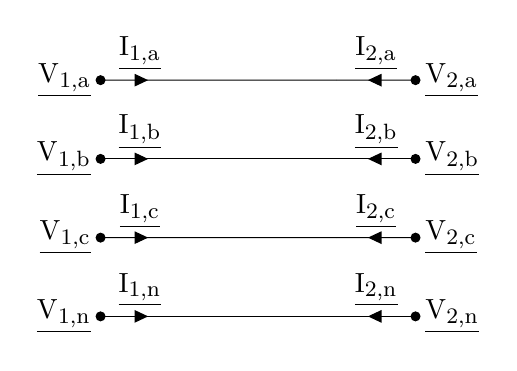
\begin{tikzpicture}[%
    show background rectangle,%
    tight background,%
    background rectangle/.style={fill=white}%
    ]
    % Version multifilaire

    %
    % Définitions
    %
    \pgfmathsetmacro{\xl}{0};%
    \pgfmathsetmacro{\xlc}{1};%
    \pgfmathsetmacro{\xrc}{3};%
    \pgfmathsetmacro{\xr}{4};%
    \pgfmathsetmacro{\yn}{0};%
    \pgfmathsetmacro{\yc}{1};%
    \pgfmathsetmacro{\yb}{2};%
    \pgfmathsetmacro{\ya}{3};%

    % Début de ligne
    \coordinate (vln) at (\xl,\yn);
    \coordinate (vlc) at (\xl,\yc);
    \coordinate (vlb) at (\xl,\yb);
    \coordinate (vla) at (\xl,\ya);

    % Fin de ligne
    \coordinate (vrn) at (\xr,\yn);
    \coordinate (vrc) at (\xr,\yc);
    \coordinate (vrb) at (\xr,\yb);
    \coordinate (vra) at (\xr,\ya);

    % Tensions amont
    \node[left] at (vla) {$\underline{V_{1,\arm}}$};
    \node[left] at (vlb) {$\underline{V_{1,\brm}}$};
    \node[left] at (vlc) {$\underline{V_{1,\crm}}$};
    \node[left] at (vln) {$\underline{V_{1,\nrm}}$};

    % Tensions aval
    \node[right] at (vra) {$\underline{V_{2,\arm}}$};
    \node[right] at (vrb) {$\underline{V_{2,\brm}}$};
    \node[right] at (vrc) {$\underline{V_{2,\crm}}$};
    \node[right] at (vrn) {$\underline{V_{2,\nrm}}$};

    % Câbles
    \draw (vla) to[short, i=$\underline{I_{1,\arm}}$, *-] (\xlc, \ya) -- (\xrc, \ya);
    \draw (vlb) to[short, i=$\underline{I_{1,\brm}}$, *-] (\xlc, \yb) -- (\xrc, \yb);
    \draw (vlc) to[short, i=$\underline{I_{1,\crm}}$, *-] (\xlc, \yc) -- (\xrc, \yc);
    \draw (vln) to[short, i=$\underline{I_{1,\nrm}}$, *-] (\xlc, \yn) -- (\xrc, \yn);

    \draw (vra) to[short, i_=$\underline{I_{2,\arm}}$, *-] (\xrc, \ya);
    \draw (vrb) to[short, i_=$\underline{I_{2,\brm}}$, *-] (\xrc, \yb);
    \draw (vrc) to[short, i_=$\underline{I_{2,\crm}}$, *-] (\xrc, \yc);
    \draw (vrn) to[short, i_=$\underline{I_{2,\nrm}}$, *-] (\xrc, \yn);

\end{tikzpicture}
\end{document}
% Local Variables:
% mode: latex
% TeX-engine: luatex
% TeX-source-correlate-method-active: synctex
% ispell-local-dictionary: "british"
% coding: utf-8
% LaTeX-indent-level: 4
% fill-column: 120
% End:
